%FOR PDFLATEX USE ONLY
\documentclass[a4paper,12pt]{article}

\usepackage{amssymb,amsmath} %math symbols

\usepackage[margin=2cm]{geometry} %paper geometry

\usepackage[T1, T2A]{fontenc}

\usepackage[utf8]{inputenc} %allows unicode (including russian) source file
\usepackage[russian]{babel} %docment in russian-style
\usepackage[utf8]{inputenc}
%\usepackage[unicode]{hyperref} %links inside of the text
\usepackage[pdftex]{graphicx} %includegraphics pictures
\usepackage{cmlgc} %bold text

\usepackage{array} %arrays

%\usepackage{wrapfig}
%\usepackage{array}
%\usepackage{lipsum}
%\usepackage{esvect}
%\usepackage{hyperref}

\usepackage{amsmath}
\usepackage{amssymb}
\usepackage{mathtools}
\usepackage{mathtext}

\usepackage{subfig}
%\usepackage{calc}
%\usepackage{pgfplots,tikz,circuitikz}
%\usepackage{tkz-euclide}
\usepackage{wrapfig}

\begin{document}

\begin{center}
  \LARGE{Работа 3.5.1}\\[0.2cm]
  \LARGE{Изучение плазмы газового разряда в неоне.}\\[0.2cm]
  \large{Малиновский Владимир}\\[0.2cm]
  \normalsize{\texttt{galqiwi@galqiwi.ru}}
\end{center}

\textbf{Цель работы:} Исследование кривых намагничивания ферромагнетиков с помощью баллистического гальванометра.\\
\textbf{В работе используются:} генератор тока с блоком питания, тороид, соленоид, баллистический гальванометр с осветителем и шкалой, амперметры, магазин сопротивлений, лабораторный автотрансформатор (ЛАТР), разделительный трансформатор.\\

\section*{Теория}
\subsection*{Плазма}
В ионизированном газе поле ионов <<экранируется>> электронами. Для поля $\mathbf{E}$ и плотности $\rho$ электрического заряда
$$
\text{div}~\mathbf{E} = 4 \pi \rho,
$$
а с учётом сферической симметрии и $\mathbf{E} = -\text{grad}~\varphi$:
\begin{equation}
\dfrac{d^2 \varphi}{dr^2}+\dfrac{2}{r}\dfrac{d\varphi}{dr}=-4\pi \rho.
\end{equation}
Плотности заряда электронов и ионов (которые мы считаем бесконечно тяжёлыми и поэтому неподвижными)
\begin{equation}
\begin{array}{c}
\rho_e = -ne \cdot \exp\left(\dfrac{e\varphi}{kT_e}\right),\\
\rho_i = ne.
\end{array}
\end{equation}
Тогда из $(1)$ в предположении $\dfrac{e\varphi}{kT_e} \ll 1$ получим
\begin{equation}
\varphi = \dfrac{Ze}{r}e^{-r/r_D},
\end{equation}
где $r_D = \sqrt{\dfrac{kT_e}{4\pi n e^2}}$ -- \textit{радиус Дебая}. Среднее число ионов в сфере такого радиуса 
\begin{wrapfigure}{r}{4cm}
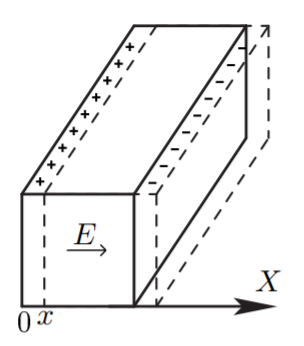
\includegraphics[scale=0.5]{2.png}
\end{wrapfigure}  
\begin{equation}
N_D = n\dfrac{4}{3}\pi r_D^2.
\end{equation}
Теперь выделим параллелепипед с плотностью $n$ электронов, сместим их на $x$. Возникнут поверхностные заряды $\sigma = nex$, поле от которых будет придавать электронам ускорение:
$$
\dfrac{d^2x}{dt^2}=-\dfrac{eE}{m}=-\dfrac{4\pi n e^2}{m}x.
$$ 
Отсюда получаем \textit{плазменную (ленгмюровскую) частоту} колебаний электронов:
\begin{equation}
\omega_p = \sqrt{\dfrac{4\pi ne^2}{m}}.
\end{equation}
\subsection*{Одиночный зонд}
При внесении в плазму уединённого проводника -- \textit{зонда} -- с потенциалом, изначально равным потенциалу точки плазмы, в которую его помещают, на него поступают токи электроннов и ионов:
\begin{equation}
\begin{array}{c}
I_{e0} = \dfrac{n \langle v_e \rangle}{4}eS,\\
I_{i0} = \dfrac{n \langle v_i \rangle}{4}eS,
\end{array}
\end{equation}
где $\langle v_e \rangle$ и $\langle v_i \rangle$ -- средние скорости электронов и ионов, $S$ -- площадь зонда, $n$ -- плотность электронов и ионов. Скорости электронов много больше скорости ионов, поэтому $I_{i0} \ll I_{e0}$. Зонд будет заряжаться до некоторого равновестного напряжения $-U_f$ -- \textit{плавающего потенциала}.\\
\begin{wrapfigure}{r}{5.5cm}
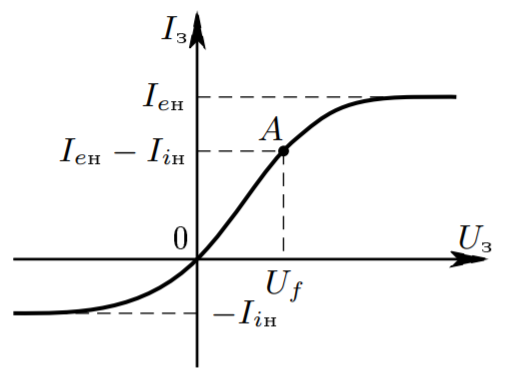
\includegraphics[scale=0.5]{3.png}
\end{wrapfigure}  
В равновесии ионный ток мало меняется, а электронный имеет вид
$$
I_e = I_0 \exp\left( -\dfrac{eU_f}{kT_e} \right).
$$
Будем подавать потенциал $U_\text{з}$ на зонд и снимать значение зондового тока $I_\text{з}$. Максимальное значение тока $I_{e\text{н}}$ -- электронный ток насыщения, а минимальное $I_{i\text{н}}$ -- ионный ток насыщения. Значение из эмпирической формулы Бомона:
\begin{equation}
I_{i\text{н}} = 0.4 neS \sqrt{\dfrac{2kT_e}{m_i}}.
\end{equation}
\subsection*{Двойной зонд}
Двойной зонд -- система из двух одинаковых зондов, расположенных на небольшом расстоянии друг от друга, между которыми создаётся разность потенциалов, меньшая $U_f$. Рассчитаем ток между ними вблизи $I=0$. При небольших разностях потенциалов ионные токи на оба зонда близки к току насыщения и компенсируют друг друга, а значит величина результирующего тока полностью связана с разностью электронных токов. Пусть потенциалы на зондах
$$
U_1 = -U_f + \Delta U_1,
$$
$$
U_2 = -U_f + \Delta U_2.
$$
Между зондами $U = U_2 - U_1 = \Delta U_2 - \Delta U_1$.
Через первый электрод
\begin{equation}
I_1 = I_{i\text{н}} + I_{e1} = I_{i\text{н}} - \dfrac{1}{4}neS\langle v_e\rangle \exp\left(-\dfrac{eU_f}{kT_e}\right)\exp\left(\dfrac{e\Delta U_1}{kT_e}\right)=I_{i\text{н}}\left(1 - \exp\left( \dfrac{e\Delta U_1}{kT_e} \right)\right).
\end{equation}
Аналогично через второй получим
\begin{equation}
I_2 = I_{i\text{н}}\left(1 - \exp\left( \dfrac{e\Delta U_2}{kT_e} \right)\right)
\end{equation}
  
Из $(7)$ и $(8)$ с учётом последовательного соединение зондов ($I_1 = -I_2 = I)$:
$$
\Delta U_1= \dfrac{kT_e}{e}\text{ln}\left(1 - \dfrac{I}{I_{i\text{н}}}\right)
$$
$$
\Delta U_2= \dfrac{kT_e}{e}\text{ln}\left(1 + \dfrac{I}{I_{i\text{н}}}\right)
$$

Тогда итоговые формулы для разности потенциалов и тока

\begin{equation}
U = \dfrac{kT_e}{e}\text{ln}\dfrac{1 - I/I_{i\text{н}}}{1 + I/I_{i\text{н}}}, 
I = I_{i\text{н}} \text{th}\dfrac{eU}{2kT_e}.
\end{equation}
Реальная зависимость выглядит несколько иначе и описывается формулой 
\begin{wrapfigure}{l}{7cm}
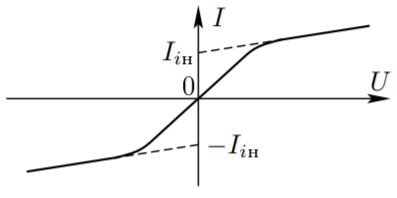
\includegraphics[scale=0.8]{4.png}
\vspace{+30pt}
\end{wrapfigure}
\begin{equation}
I = I_{i\text{н}} \text{th}\dfrac{eU}{2kT_e} + AU.
\end{equation}
Из этой формулы можно найти формулу для $T_e$: для $U=0$ мы найдём $I_{i\text{н}}$, продифференцируем в точке $U=0$ и с учётом $\text{th}~\alpha \approx \alpha$ при малых $\alpha$ и $A\rightarrow 0$ получим:
\begin{equation}
kT_e = \dfrac{1}{2}\dfrac{eI_{i\text{н}}}{\dfrac{dI}{dU}|_{U=0}}.
\end{equation}
\section*{Описание установки}
\begin{center}
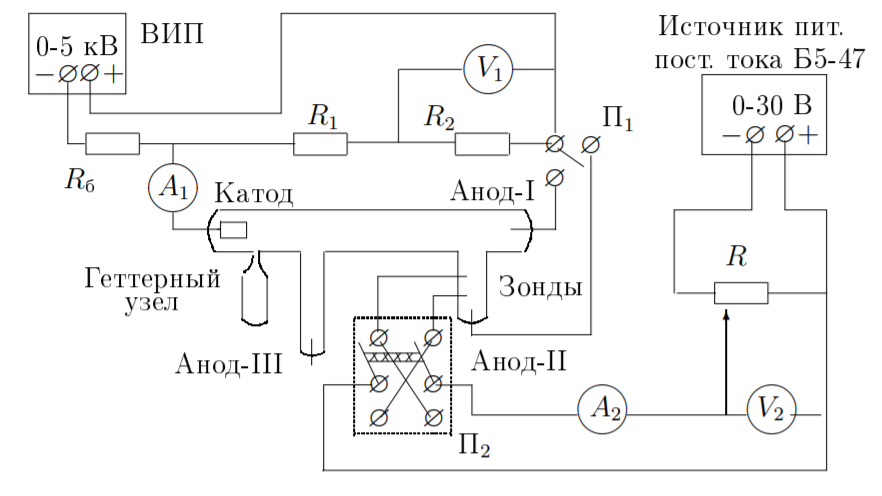
\includegraphics[scale=0.6]{1.png}
\end{center}
Стеклянная газоразрядная трубка имеет холодный (ненакаливаемый) полый катод, три анода и \textit{геттерный} узел -- стеклянный баллон, на внутреннюю повехность которого напылена газопоглощающая плёнка (\textit{геттер}). Трубка наполнена изотопом неона $^22$Ne при давлении 2 мм рт. ст. Катод и один из анодом (I и II) с помощью переключателя $\Pi_1$ подключается через балластный резистор $R_\text{б}$ ($\approx 450$ кОм) к регулируемому ВИП с выкодным напряжением до 5 кВ.\\
При подключении к ВИП анода-I между ним и катодом возникает газовый разряд. Ток разряда измеряется миллиамперметром $A_1$, а падение напряжения на разрядной трубке -- цифровым вольтметром $V_1$, подключённым к трубке черезе высокоомный (25 МОм) делитель напряжения с коэффициентом $(R_1+R_2)/R_2 = 10$.\\
При подключении к ВИП анода-II разряд возникает в пространстве между катодом и анодом-II, где находятся двойной зонд, используемый для диагностики плазмы положительного столба. Зонды изготовлены из молибденовой проволоки диаметром $d = 0.2$ мм и имеют длину $l = 5.2$ мм. Они подключены к источнику питания GPS через потенциометр $R$. Переключатель $\Pi_2$ позволяет изменять полярность напряжения на зондах. Величина напряжения на зондах изменяеься с помощью дискретного переключателя <<$V$>> выходного напряжения источника питания и потенциометра $R$, а измеряется цифровым вольтметром $V_2$. Для измерения зондового тока используется мультиметр $A_2$.
\section*{Ход работы}
Измеряем напряжение зажигания в лампе: $U_{\text{заж}} = 20.4\pm 0.2$ В.\\
С помощью вольтметра $V_1$ и амперметра $A_1$ снимаем ВАХ разряда $U_1=f(I_p)$ для тока в диапазоне $0.5 \div 5$ мА (см. Таблица 1).
Построим график:\\
\begin{center}
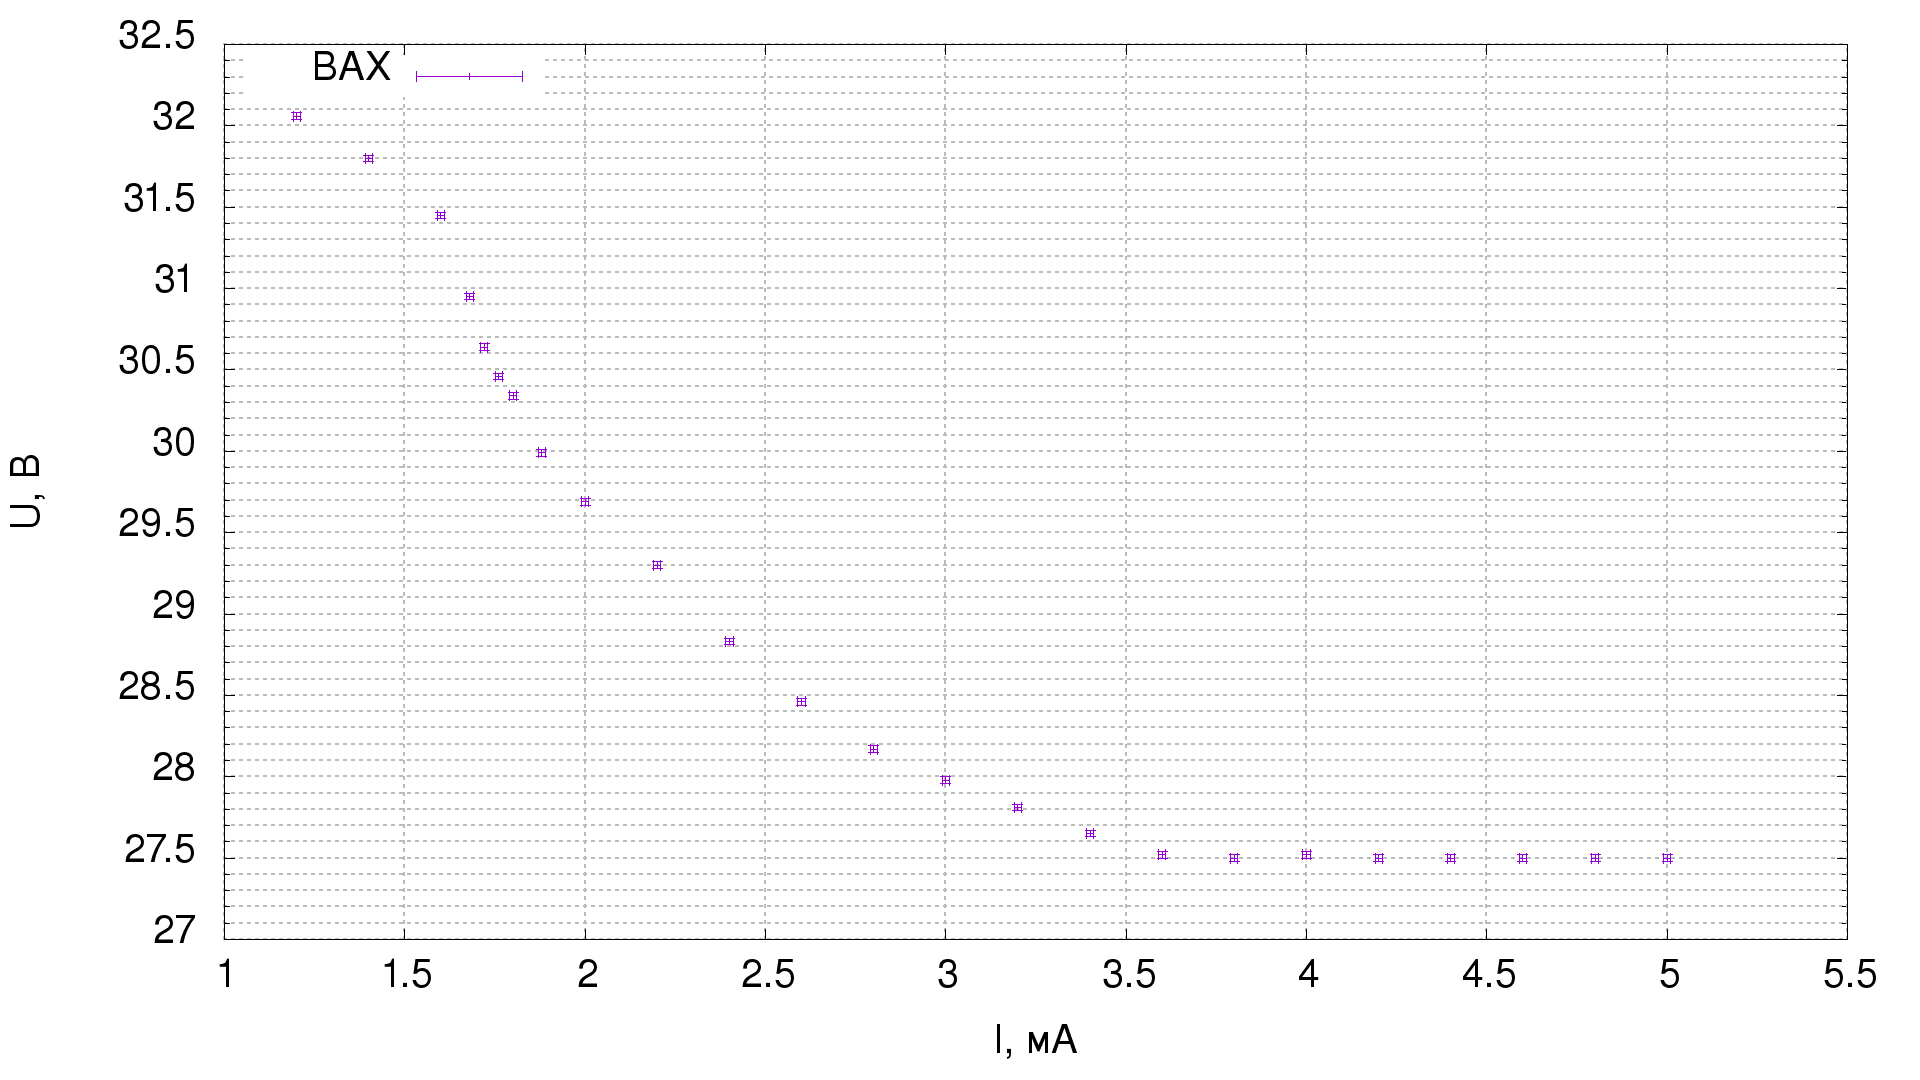
\includegraphics[width=0.95\textwidth]{iu.png}
Вольт-амперная характеристика разряда.
\end{center}
<написать рпо максимальное сопротивление>\\
С помощью вольтмертра $V_2$ и амперметра $A_2$ снимем ВАХ двойного зонда $I_2 = f(U_2)$ при фиксированного токе разряда $I_p$ в трубке в диапозоне $-25 \div 25$ В, процессе измерений меняя полярность зонда при нулевом токе. Измерения проведём для $I_p = 5$ мА, $I_p = 3$ мА  и $I_p = 1.5$ мА.\\
Используя МНК, найдем коэффициенты в формуле тока через двойной зонд от напряжения:
$$I = I_{in}\,th(BU) + AU.$$
Из него вычислим $I_in$ и $kT_e$, используя формулу
$$B=\frac{e}{2kT_e}.$$
Также найдем концентрацию ионов $n_e$ из формулы $I_{in} = 0.4 n_e e S \sqrt{\frac{2kT_e}{m_i}}$, дебаевский радиус $r_D$, число электронов в дебаевской сфере $N_D$ и степень ионизации плазмы $\alpha$.

\begin{center}
\begin{tabular}{|c|c|c|c|c|c|c|}\hline
$I_{in}$, мкА&$T_e$, эВ&$n_e$, $10^{16}$ $\text{м}^{-3}$&$\omega_p$, $10^{25} \text{рад}/\text{с}$&$N_D, 10^5$&$\alpha, 10^{-7}$\\ \hline
$105.4\pm0.2$ &$4.97\pm0.06$&$7.64\pm0.09$&$4.32\pm0.05$&$26\pm1$&$3.16\pm0.04$\\ \hline
$47.9\pm0.1$  &$3.73\pm0.06$&$3.73\pm0.06$&$5.97\pm0.09$&$36\pm1$&$1.66\pm0.03$\\ \hline
$24.41\pm0.02$&$3.68\pm0.06$&$2.06\pm0.03$&$8.34\pm0.13$&$50\pm1$&$0.85\pm0.01$\\ \hline
\end{tabular}
\end{center}

\begin{center}
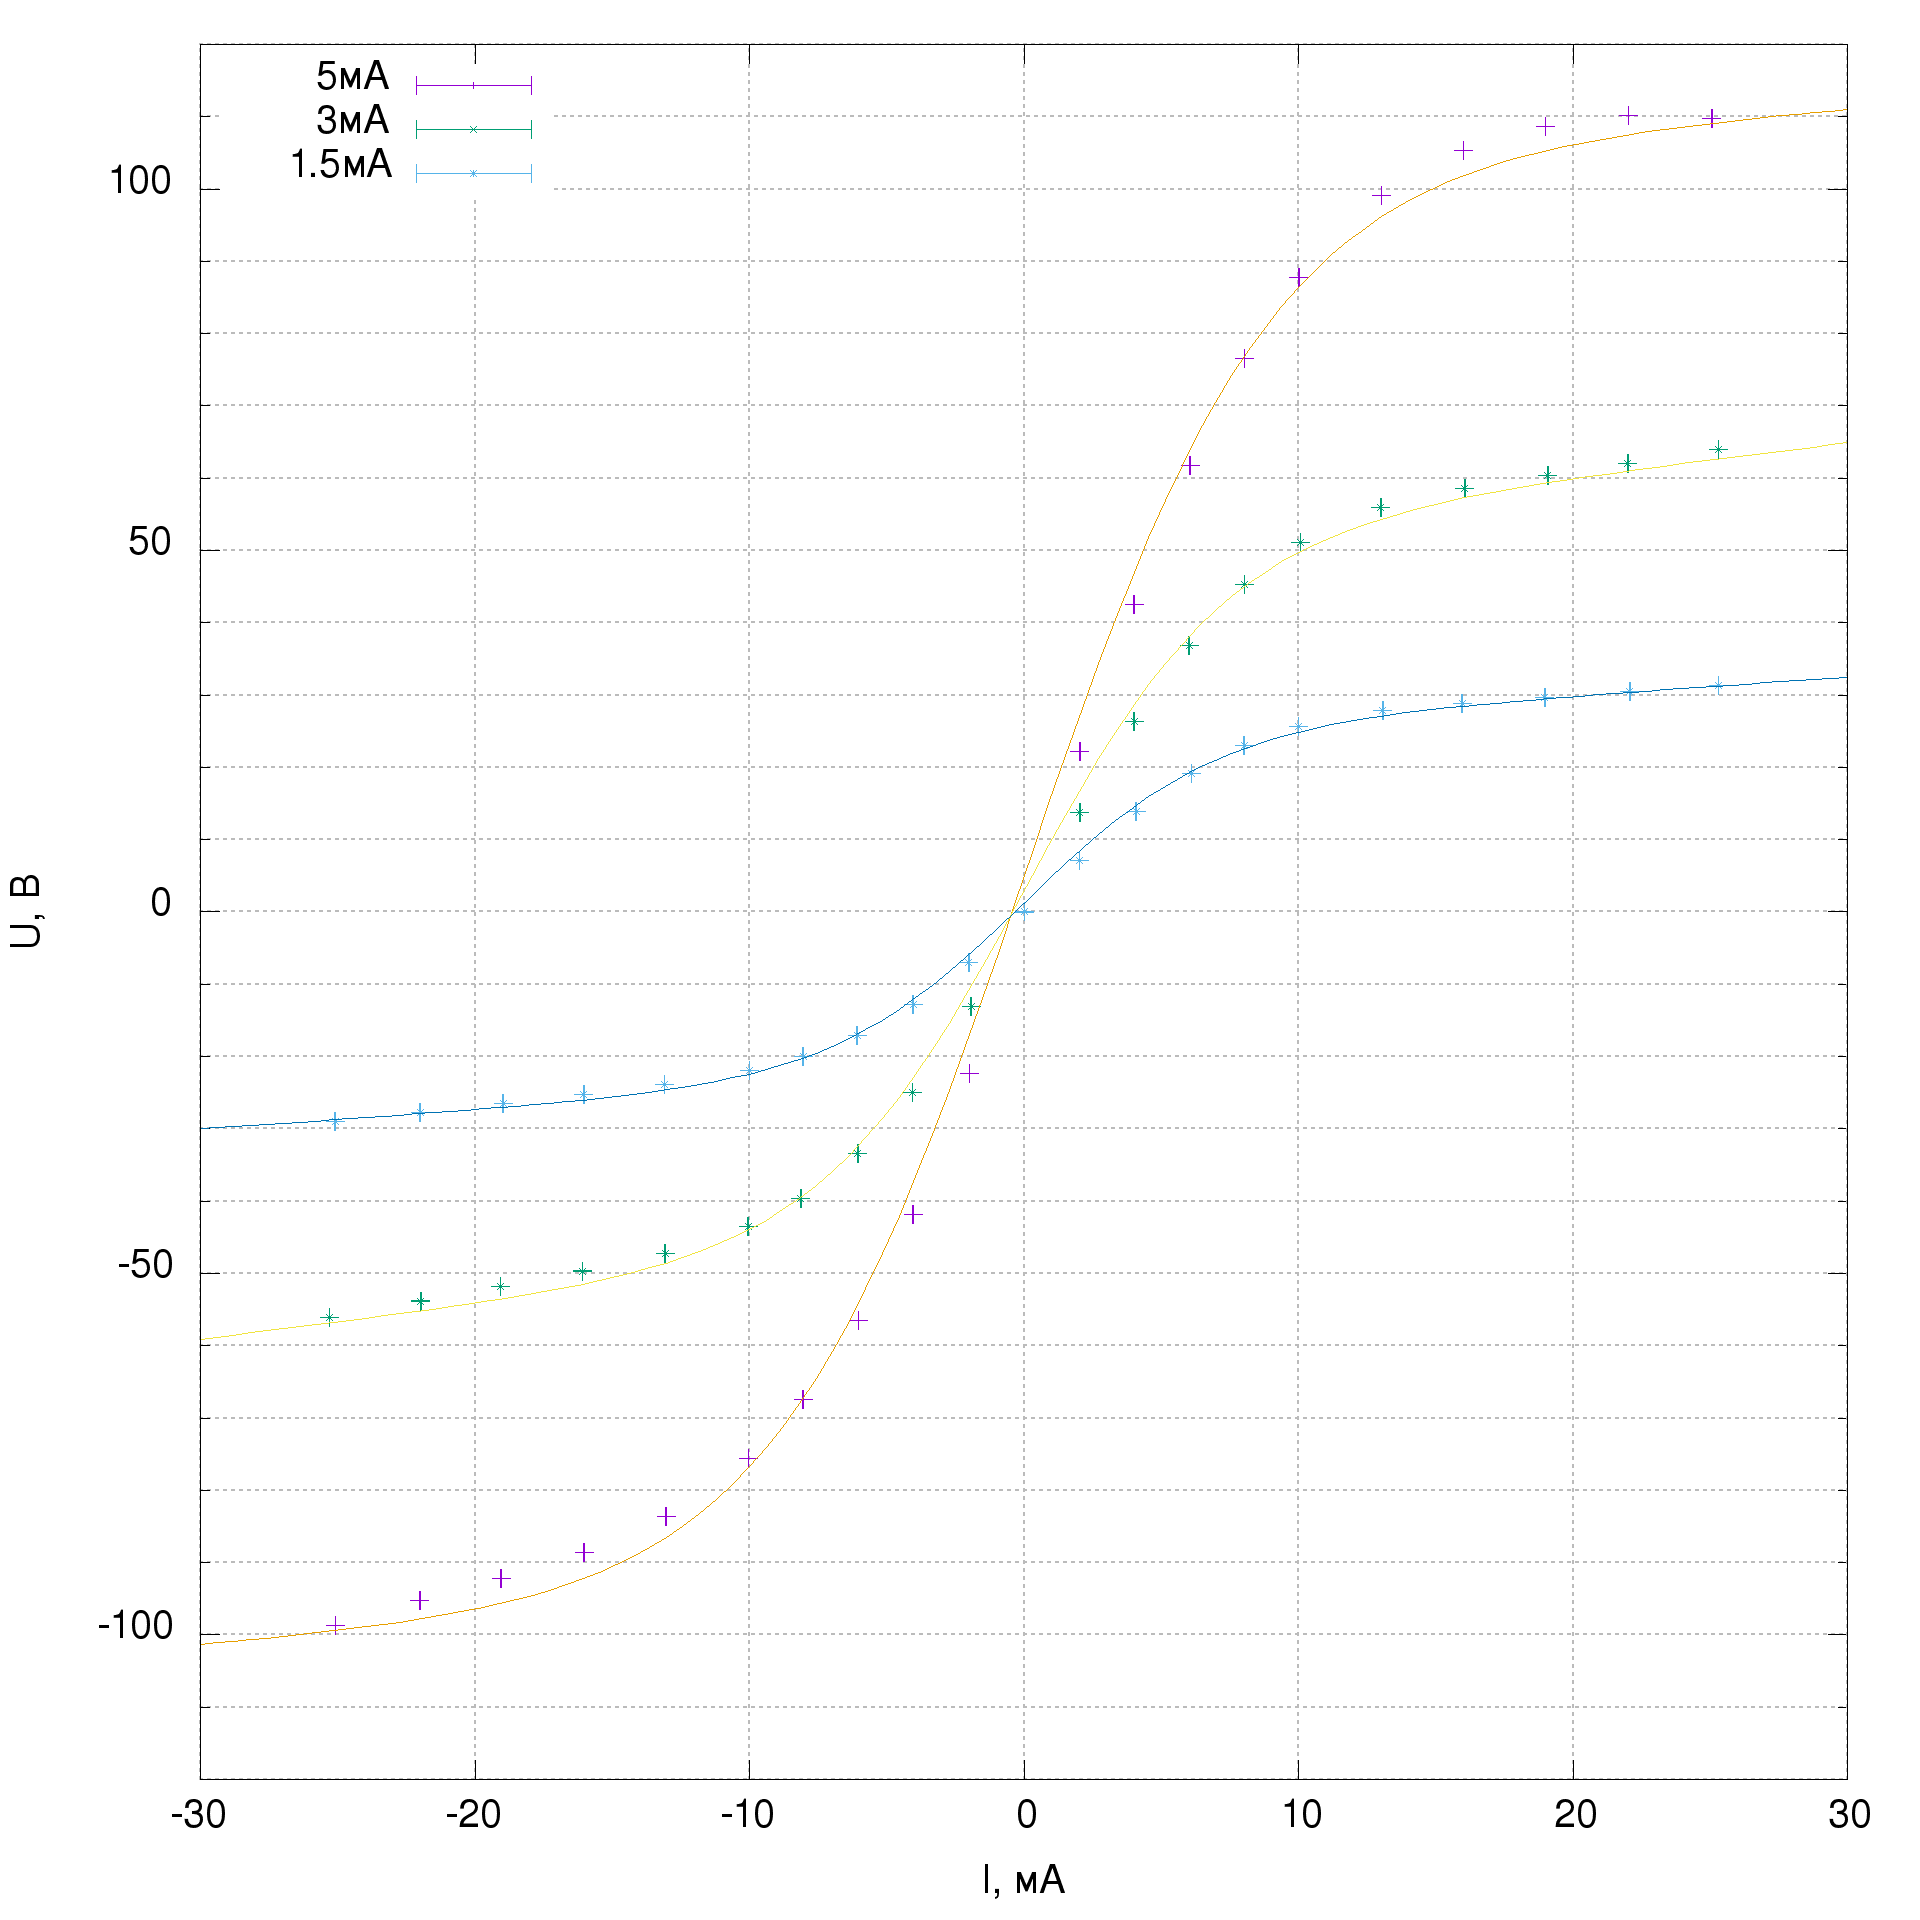
\includegraphics[width=0.95\textwidth]{iu2.png}
Вольт-амперная характеристика разряда.
\end{center}

\section*{Вывод}
В данном эксперименте проводилось изучение ВАХ плазменного разряда и двойного зонда, находящегося в ней. Все зависимости имеют вид, предсказанный теорией, а полученные результаты совпадают с табличными.

\end{document}








\lipsum[1-4]
\begin{wrapfigure}{R}{5cm}
\centering
\includegraphics[width=0.20\textwidth]{rd.png}
\caption{1}
\end{wrapfigure}
\lipsum[1-6]


\begin{figure}[h]
\begin{center}$
\begin{array}{cccc}
\includegraphics[width=0.20\textwidth]{rd.png}&
\includegraphics[width=0.20\textwidth]{rd.png}&
\includegraphics[width=0.20\textwidth]{rd.png}&
\includegraphics[width=0.20\textwidth]{rd.png}\\
(1) & (2) & (3) & (4)
\end{array}$
\end{center}
\end{figure}
